\documentclass[11pt]{article}
\usepackage[a4paper, portrait, margin=1in]{geometry}
\usepackage{graphicx}


\begin{document}

\title{Advanced Systems Lab (Fall'15) -- First
Milestone}

\author{Name: \emph{Marcel Mohler}\\Legi number: \emph{09-922-998}}

\date{
\vspace{4cm}
\textbf{Grading} \\
\begin{tabular}{|c|c|}
\hline  \textbf{Section} & \textbf{Points} \\ 
\hline  1.1 &  \\ 
\hline  1.2 &  \\ 
\hline  1.3 &  \\ 
\hline  2.1 &  \\ 
\hline  2.2 &  \\ 
\hline  2.3 &  \\ 
\hline  3.1 &  \\ 
\hline  3.2 &  \\ 
\hline  3.3 &  \\ 
\hline  3.4 &  \\ 
\hline  3.5 &  \\ 
\hline  3.6 &  \\ 
\hline \hline Total & \\
\hline 
\end{tabular} 
}

\maketitle

\newpage

\section{System Description}\label{sec:system-description}

\subsection{Database}\label{sec:database}

Length: 1-2 pages

Start by explaining the schema of the database and the indexes used to
speed up data access. Describe the interface to the database (queries
and stored procedures).

Make sure to explain the design in terms of what you wanted to achieve,
what decisions you took and what is the expected behavior.

Include baseline performance characteristics of the database (max
throughput, response time, and scalability).

\subsubsection{Schema and Indexes}\label{sec:schema-and-indexes}
Our goal was to keep the database schema as simple as possible to avoid the need of complex queries. In the absence of costly table join operations, we hope to achieve a more predictable database performance without the need to worry about heavy database optimizations. The layout is depicted in Figure \ref{fig:dbschema}. The id of \texttt{queues} and \texttt{clients} pose a foreign key constraint to the \texttt{messages} table. This means that it is not possible to insert a message with a sender, receiver or queue id that does not exist in the database.\\
Since we want to be able to efficiently delete clients and queues we created an index on id in both \texttt{clients} and \texttt{queues}.
On the \texttt{messages} table indexes on id (\texttt{pop\_queue()}), queue\_id (\texttt{pop\_queue()}, \texttt{peek\_queue()}), sender\_id (\texttt{pop\_message()}) and receiver\_id (\texttt{pop\_queue()}, \texttt{peek\_queue()}, \texttt{pop\_message()}) were created to allow performant selection on these columns. The brackets denote the queries that profit from these indexes which are described in more detail in section \ref{sec:stored-procedures}.
\begin{figure}
  \begin{center}
    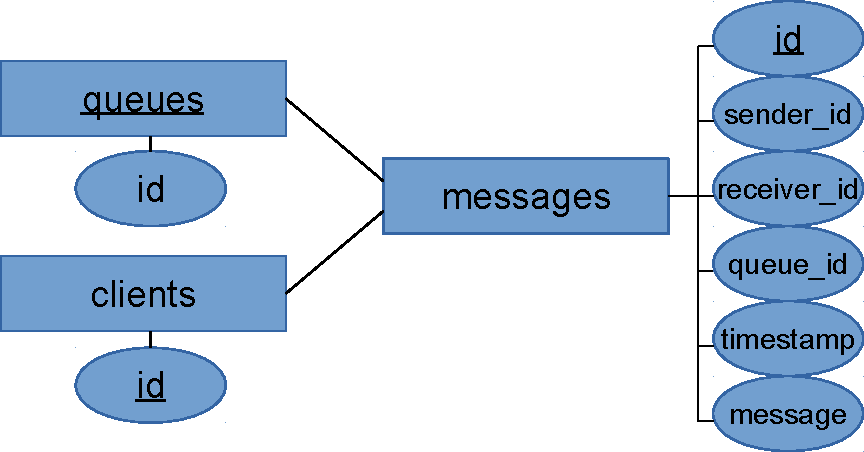
\includegraphics[width=0.6\textwidth]{figures/dbschema.pdf}
    \caption{DB schema}
    \label{fig:dbschema}
  \end{center}
\end{figure}

\subsubsection{Stored Procedures}\label{sec:stored-procedures}
Table \ref{tab:storedprocedures} describes the stored procedures used in SimpleMQ. The arguments client, sender, receiver, queue denote a particular client or queue id.
\begin{table}[ht]
  \caption{stored procedures in SimpleMQ}
  \label{tab:storedprocedures}
  \begin{center}
    \begin{tabular}{|p{5cm}|p{6cm}|p{1.8cm}|}
       \hline
       \textbf{stored procedure name} & \textbf{description} & \textbf{returns}\\ \hline
       add\_message(sender, receiver, queue, timestamp, message) & adds a new message & msg\_id auto-inc\\ \hline
       add\_queue() & adds a new queue & queue\_id auto-inc\\ \hline
       delete\_queue(queue) & deletes the queue & nothing\\ \hline
       query\_queues(client) & queries for a queue where messages for the client are waiting & queue\_id\\ \hline
       add\_client(client) & add a new client & nothing\\ \hline
       delete\_client(client) & deletes the client & nothing\\ \hline
       pop\_message(sender, receiver) & reads and removes the oldest message from a particular sender & message\\ \hline
       pop\_queue(queue, receiver) & reads and removes the oldest message for a particular receiver & message\\ \hline
       peek\_queue(queue, receiver) & reads the oldest message for a particular receiver & message\\ \hline
    \end{tabular}
  \end{center}
\end{table}
\subsubsection{Design decisions}\label{sec:design-decisions}
While the simplicity of the schema favors the ability to write basic queries, we expect this to have an negative influence on performance.
In particular, apart from clients and queue creation/deletion, all queries operate on the single table \texttt{messages}. This means that when multiple middlewares access the database concurrently, the database has to deploy locking mechanisms to prevent concurrency artifacts like dirty reads, lost updates or phantoms \footnote{see ETH Lecture Information Systems: https://globis.ethz.ch/files/2015/04/IS-lect14-concurrency.pdf}.
\subsubsection{Performance characteristics}\label{sec:performance-characteristics}

\subsection{Middleware}\label{sec:middleware}

Length: 1-2 pages

Explain the design from a high-level point of view, highlighting what
you wanted to achieve, design decisions, expected behavior.

Then go into more detail on how the middleware connects to the database
and clients, and how queuing is implemented.

Show what are the performance characteristics of the middleware
(i.e.~throughput, latency, scalability).

\subsubsection{Design overview}\label{sec:design-overview}
The main goal was to provide a middleware, that scales well, when increasing the number of clients. This means that we expect the system throughput to be constant once the middleware receives the maximum number of requests it can support. This quantity is determined by the amount of internal worker threads which is proportional to the amount of possible connections to the database.
Adding more clients to the system should not negatively impact performance but at the same time no clients should suffer from starvation.
\\
To allow asynchronous requests we have chosen to implement the middleware using Java NIO.
\\
Each middleware instance basically consists of two major components: one distributor and multiple worker threads.
The distributor iterates over incoming requests (also called \textit{key} in Java NIO) and distributes these requests to the workers. Available workers are stored in a concurrent blocking queue. This means that in case no worker is available, the distributor will wait until a worker finishes. The total amount of workers is a configurable parameter.



\subsubsection{Interfacing with clients}\label{sec:interfacing-with-clients}
The middleware provides a ServerSocket on a predefined port. Clients can send requests to that port and the server will handle them eventually (asynchronously).
Clients need to start by issueing a \texttt{CreateClient} request. The middleware then contacts the database to insert the clients ID. As soon as a client sends a \texttt{DeleteClient} request, the middleware deletes its ID from the database.
The requests and answers are serialized Java classes, defined in a shared API.

\subsubsection{Queuing and Connection pool to database}\label{sec:queuing-and-connection-pool-to-database}
Every worker maintains a persistent connection to the database. In our experiments we always make sure that we do not have more workers than the amount of simultaneous connections the database accepts.
\subsubsection{Performance characteristics}\label{sec:performance-characteristics-1}

\subsection{Clients}\label{sec:clients}

Length: 2-3 pages

Explain the interface of the clients to your messaging system and their
high level design, including the ways you have instrumented the code for
debugging and benchmarking purposes.

Provide a detailed description of the workloads used later in the report
(operation mix, starting and ending state of the database, assumptions
on workload behavior). Explain how the load was generated (include
baselines on load generation speed) and how the clients were deployed.

Which are the sanity checks in place for ensuring correct load
generation and validity of responses?

\subsubsection{Design and interface}\label{sec:design-and-interface}
The clients are designed as simple as possible. They basically 
\subsubsection{Instrumentation}\label{sec:instrumentation}
Each client keeps a log of all outgoing requests and incoming answers.
\subsubsection{Workloads and deployment}\label{sec:workloads-and-deployment}

Clients were deployed on AWS micro instances. To provide reliable results it is important we measure the maximum number of clients a single instance can host before the instance's CPU and memory empose a limit on additional clients. This allows us to later scale up the clients without having to worry about their local performance. If we simply increase the number of clients per instance it can happen that the system would actually be able to handle more clients but the instance itself limits the clients to handle more messages.
For this system we chose large AWS instances for database and server to make sure they do not limit the system and handle client requests immediately. We are aware, that this might not be the case when the system is under heavy load, but this will only result in less message answers for the clients to handle and therefore even less work on the client instances. We therefore seek the maximum number of clients which an instance can handle under these ideal circumstances.
We measure the throughput and reponse time. We expect the throughput to increase with the number of clients up to a saturation level. The response time should remain on a constant level since we limit the worker at 64 (so there should always be at least one free worker on the server). We use one and two servers and conduct a $2^k$ analysis.
A visualization of our hypothesis and the results can be found in Figure \ref{fig:maxclientperinstance}.

\subsubsection{Sanity checks}\label{sec:sanity-checks}
The clients are designed as a closed loop system. They only issue the next request when they have received the previous answer.
We use a fixed 
\section{Experimental Setup}\label{sec:experimental-setup}

Length: 1-2 pages

Explain the overall design of the complete system and list the
configurations (number of middlewares, number of clients, types of
machines, communication patterns) corresponding to the main workloads.

Describe the mechanisms for deploying the system for experiments and the
way performance numbers are gathered and processed. Make the description
so that someone unfamiliar with your system can replicate the steps, and
reference the different script files you submit as code in the SVN
repository.

\subsection{System Configurations}\label{sec:system-configurations}

\subsection{Configuration and Deployment mechanisms}\label{sec:configuration-and-deployment-mechanisms}
We tried to automate the deployment mechanisms as much as possible. Several scripts were written to achieve this goal.
\begin{itemize}
  \item \texttt{experiment.sh:} This script makes sure all instances are running the latest versions, runs the benchmarks and gathers the results. It runs locally and uses amazon instance IP's as arguments. In particular the steps are: \\1. parse command line parameter \\2. build server and client from source into a .jar using ant \\3. check if passwordless login is enabled \\4. cleanup servers in case some old experiments are still running \\5. copy compiled .jar's to client and server instances \\6. setup postgres \\7. run database, server and clients remotely \\8. wait for the clients to finish \\9. shutdown database and server \\10. copy log files from remote locations \\11. invoke further processing of log files
  \item \texttt{client.sh:} Helper script to run individual clients on the client instances. This prevents the need of keeping alive a connection to each individual client.
  \item \texttt{graphs.py:} 
\end{itemize}
\subsection{Logging and Benchmarking mechanisms}\label{sec:logging-and-benchmarking-mechanisms}

\section{Evaluation}\label{sec:evaluation}

Length: up to 10 pages

In this section we expect to see the different experiments you ran to
exercise the system, and with each experiment we expect a clear
description of the system configuration used, the hypothesis on behavior
and the explanation of the behavior observed (in terms of the different
design decisions taken beforehand) -- \emph{missing either of these for
an experiment might make you lose all points for that given experiment!}
Keep in mind that for a good explanation of the results of an experiment
you might have to use one or more methods of data analysis presented in
the lecture and in the book.

See below for a short description on what each part should contain.

\subsection{System Stability}\label{sec:system-stability}

% To prove that your system functions correctly and that it is stable
% include the trace of a 30 minute run, plotting both response time and
% throughput. Use at least 30 clients (sending and receiving data), 2
% middlewares and a non-empty database.
To show the stability of the system we let the system running for 1980 seconds (33 minutes). We use 30 clients on a single instance and two middleware servers with 32 workers each. The database contains 5000 messages from previous experiments.\\
We cut out the first minute to eliminate warmup effects.
The trace of the throughput is shown in Figure \ref{fig:throughput30min}, the response time over time is plotted in \ref{fig:response30min}.
\begin{figure}
  \begin{center}
    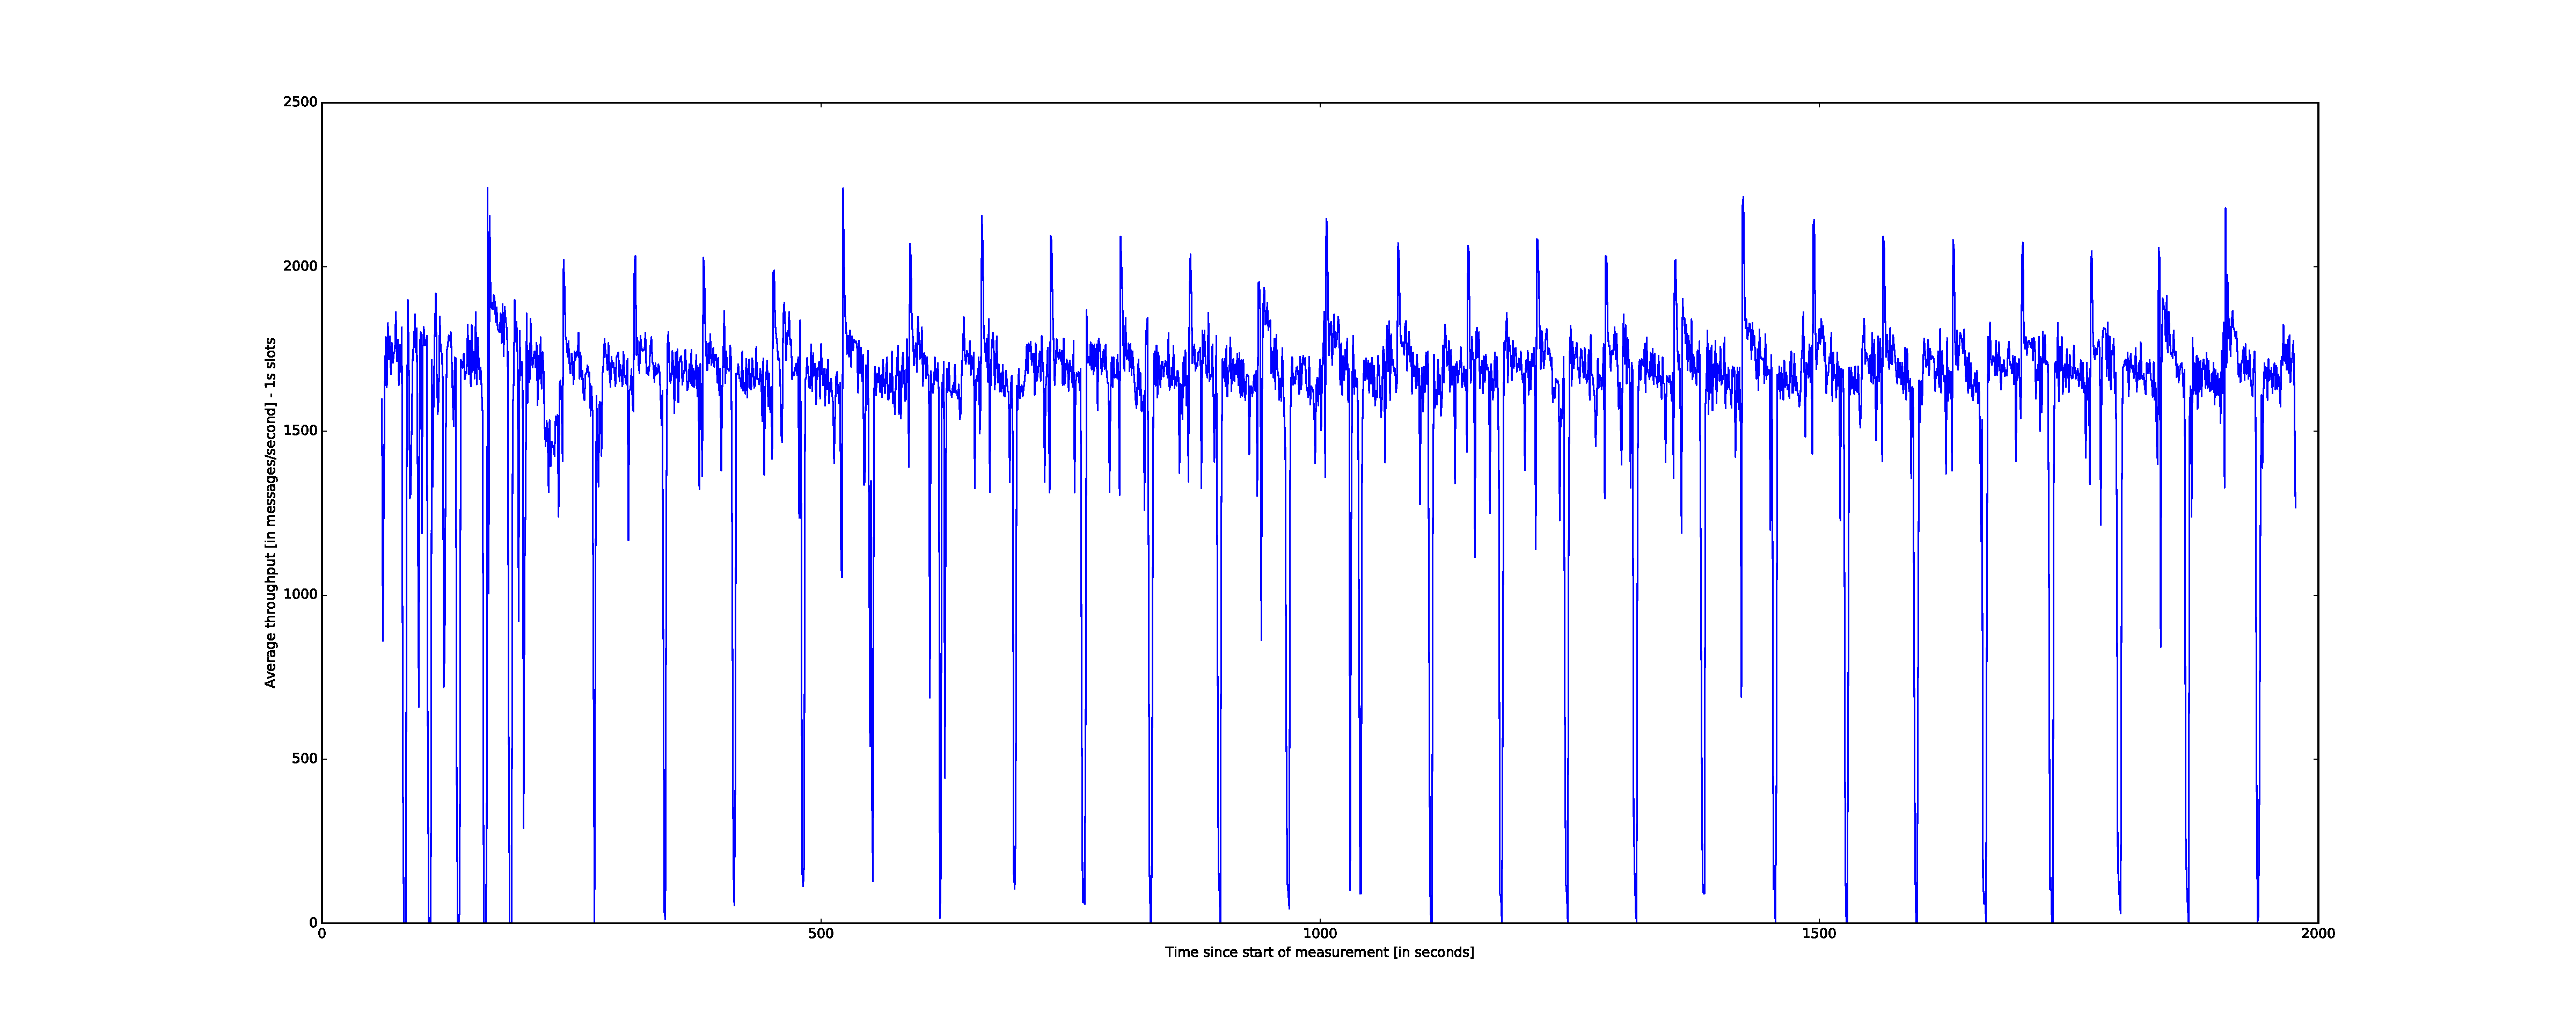
\includegraphics[width=0.5\textwidth]{../results/30min_small_throughput.pdf}
    \caption{}
    \label{fig:throughput30min}
  \end{center}
\end{figure}
\begin{figure}
  \begin{center}
    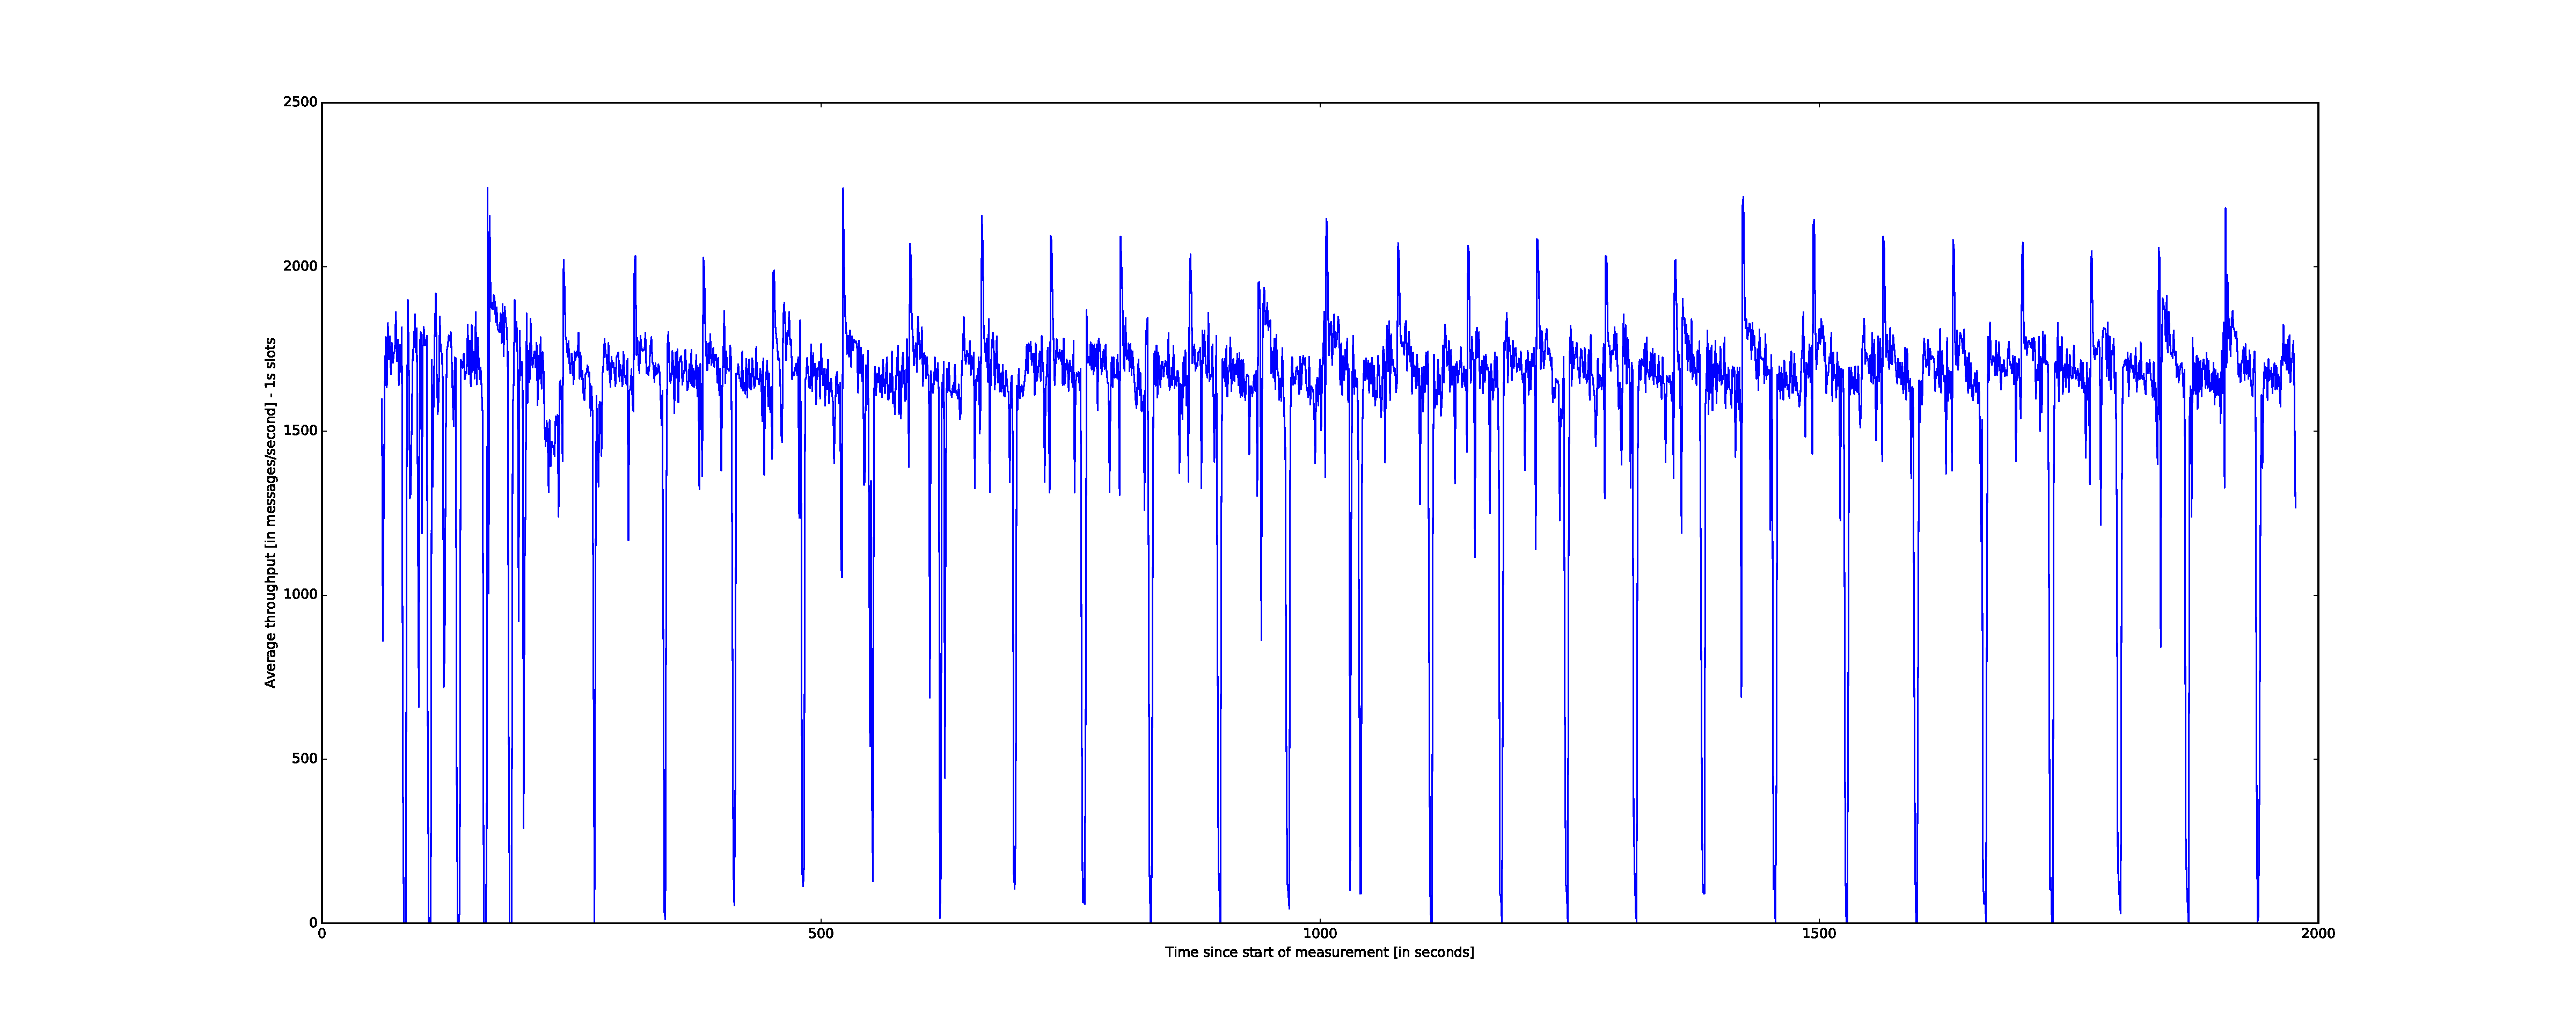
\includegraphics[width=0.5\textwidth]{../results/30min_small_throughput.pdf}
    \caption{}
    \label{fig:response30min}
  \end{center}
\end{figure}

\subsection{System Throughput}\label{sec:system-throughput}

Measure the maximum throughput of the system (describe the exact
configuration and workload, and the reasoning behind choosing these
particular ones) and show the average response time for this experiment.

\subsection{System Scalability}\label{sec:system-scalability}

We start by doing the following two experiments:
\begin{enumerate}
  \item Fix the number of workers and scale the clients
  \item Fix the number of clients and scale the workers
\end{enumerate}
We expect these experiment to give us evidence how the system behaves when we increase either resource, but limit the other. Detailed hypotheses are provided on each experiment individually below.
\subsubsection{Fix workers - scale clients}
First, we fix the number of workers to 60 and 
\begin{figure}
  \begin{center}
    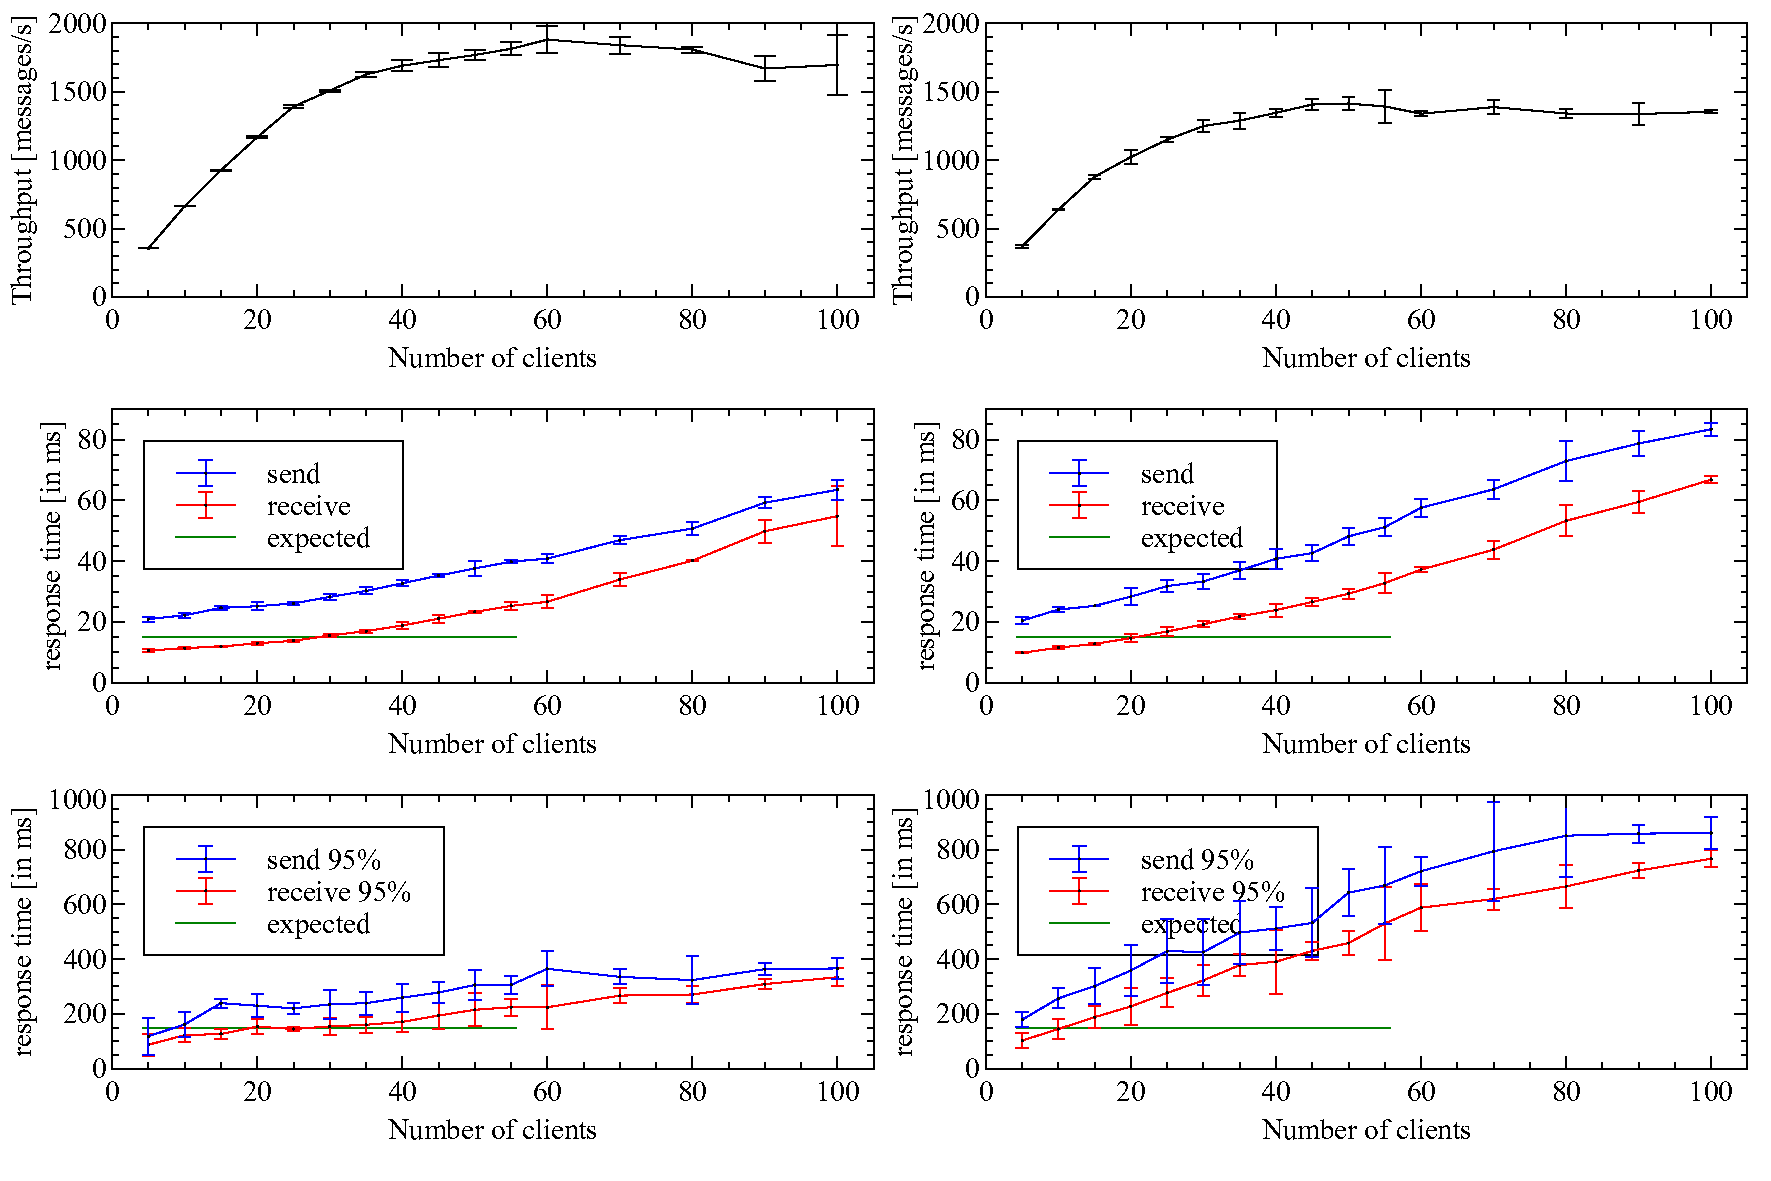
\includegraphics[width=0.9\textwidth]{../results/maxclientperinstance.pdf}
    \caption{Scaling the number of clients - left small, right large messages}
    \label{fig:maxclientperinstance}
  \end{center}
\end{figure}
\subsubsection{Fix clients - scale workers}
\begin{figure}
  \begin{center}
    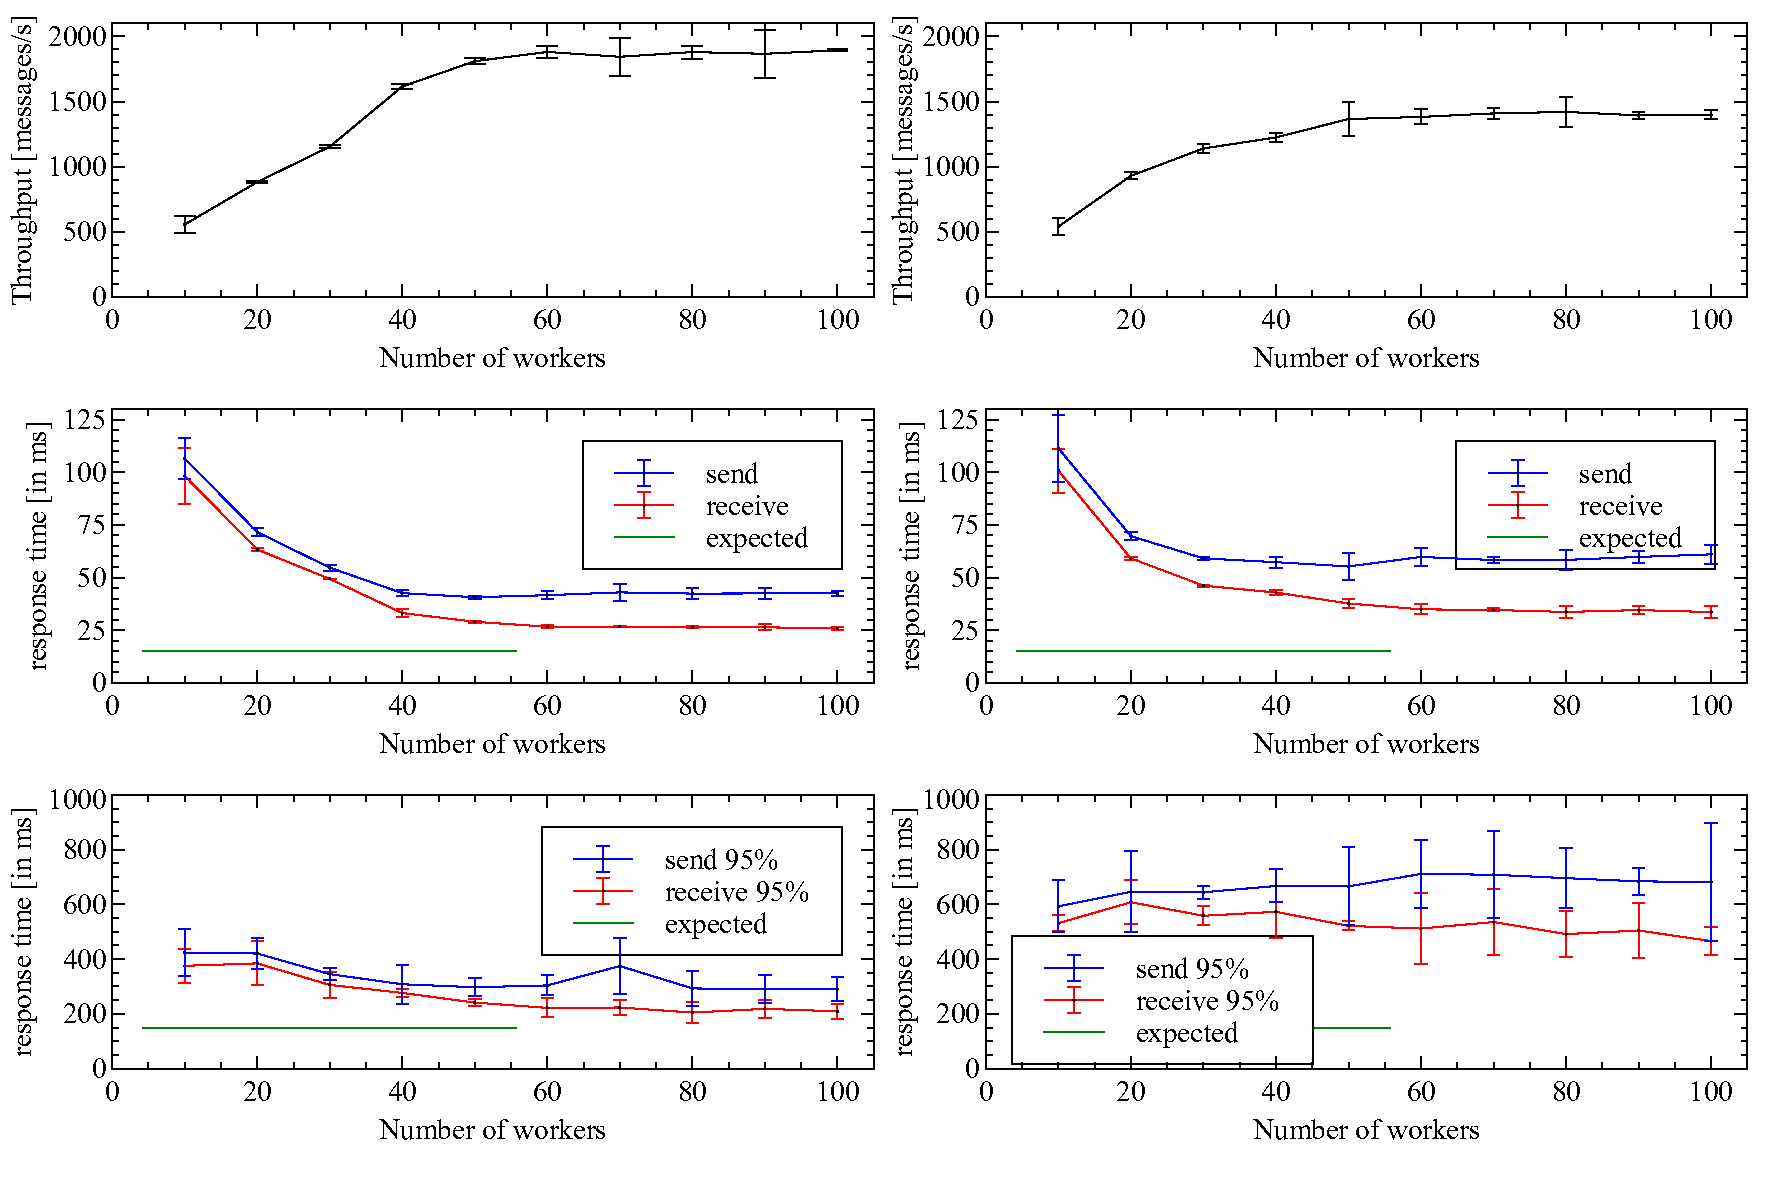
\includegraphics[width=0.9\textwidth]{../results/maxworkerperinstance.pdf}
    \caption{Scaling the number of workers - left small, right large messages}
    \label{fig:maxworkerperinstance}
  \end{center}
\end{figure}
Explain the different configurations used to explore the scalability of
your system, and the outcomes of these experiments in terms of
throughput and response times. The main goal of this subsection is to
define the ranges in which your system operates best.

\subsection{Response Time Variations}\label{sec:response-time-variations}

Report and analyze how the response times change in the system with
different message sizes, different number of clients and different
number of middleware nodes.

\subsection{$2^k$ Experiment}\label{sec:k-experiment}

Conduct a 2\^{}k analysis of your system (aim at exploring non-obvious
interactions of parameters). Use the methods learned in this lecture to
conduct the detailed analysis.

\subsection{Conclusion}\label{sec:conclusion}

To conclude the report summarize the behavior of the system in terms of
the design and the representative workloads. Finally, outline in a few
points what would you do differently if you could design the system
anew.

\end{document}
